% Latex template: https://github.com/mqTeXUsers/Macquarie-University-Beamer-Theme

% Slide Masters:

% Title
% Text
% 2 column
% Full-image
% Bibliography
% Closing
 
\documentclass[aspectratio=169, 11pt]{beamer} % Aspect ratio
% https://tex.stackexchange.com/a/14339/5483 
% Possible values: 1610, 169, 149, 54, 43 and 32.
% 169 = 16:9

\PassOptionsToPackage{table}{xcolor}    %https://tex.stackexchange.com/a/5365/5483

\usetheme{macquarie}
\usepackage{multicol} % https://tex.stackexchange.com/a/396018/5483
\usepackage{xurl}
\usepackage[british]{babel}       % Set language
% \usepackage[utf8x]{inputenc}      % Set encoding
\usepackage{colortbl}
\mode<presentation>           % Set options
{
  \usetheme{default}          % Set theme
  \usecolortheme{default}         % Set colors
  \usefonttheme{default}          % Set font theme
  \setbeamertemplate{caption}[numbered] % Set caption to be numbered
}

% Uncomment this to have the outline at the beginning of each section highlighted.
%\AtBeginSection[]
%{
%  \begin{frame}{Outline}
%    \tableofcontents[currentsection]
%  \end{frame}
%}

\usepackage{graphicx}         % For including figures
\usepackage{booktabs}         % For table rules
\usepackage{hyperref}         % For cross-referencing


\usepackage{enumitem} % https://tex.stackexchange.com/a/2292/5483

%https://tex.stackexchange.com/a/371844/5483
\setbeamerfont{bibliography entry author}{size=\tiny}
\setbeamerfont{bibliography entry title}{size=\tiny}
\setbeamerfont{bibliography entry location}{size=\tiny}
\setbeamerfont{bibliography entry note}{size=\tiny}
\setbeamerfont{bibliography item}{size=\tiny}

%https://tex.stackexchange.com/q/333587/5483
%TODO SHAWN REPLACE OSF URL
%\setbeamertemplate{footline}{\strut~\texttt{https://osf.io/v5jp7/}\hfill\insertframen%umber~/~\inserttotalframenumber\strut~~~}

\usepackage{comment} % for commenting out multiple lines; uses \begin{comment} ... \end{comment}

\title{Bringing FAIR data to Humanities research} % Presentation title
\author{A/Prof Shawn A Ross, Director of Data Science and eResearch}               % Presentation author
\institute{Office of the Deputy Vice-Chancellor (Research)}         % Author affiliation
\date{Thursday 14 May 2020}                 % Today's date  
\begin{document}

% Title page
% This page includes the information defined earlier including title, author/s, affiliation/s and the date
% \begin{frame}[noframenumbering]

\maketitle

  
% \end{frame}

% Outline
% This page includes the outline (Table of content) of the presentation. All sections and subsections will appear in the outline by default.
\begin{frame}{The context of Research Data Management}
  \tableofcontents
\end{frame}

% The following is the most frequently used slide types in beamer
% The slide structure is as follows:
%
%\begin{frame}{<slide-title>}
% <content>
%\end{frame}


% Presentation providing context for the new data governance policies and procedures at Macquarie University

\section{Why should we care about FAIR data?}

\begin{frame}{It started with the `reproducibility crisis'}
  For nearly a decade the reproducibility crisis has featured in the scientific literature \cite{Jasny2011-bw, Baker2016-cf, Munafo2017-bj}. Low reproducibility rates have emerged from large-scale studies:
    \begin{itemize}[label=\textbullet]
        \item Results from only 39\% of psychology studies could be reproduced \cite{Open_Science_Collaboration2015-vf}.
        \item Even lower reproducibility rate in biomedical research \cite{Begley2012-xt,Prinz2011-za}.
    \end{itemize}
\end{frame}

\begin{frame}{Perceptions of a crisis}
  \begin{figure}[H]
    \centering
        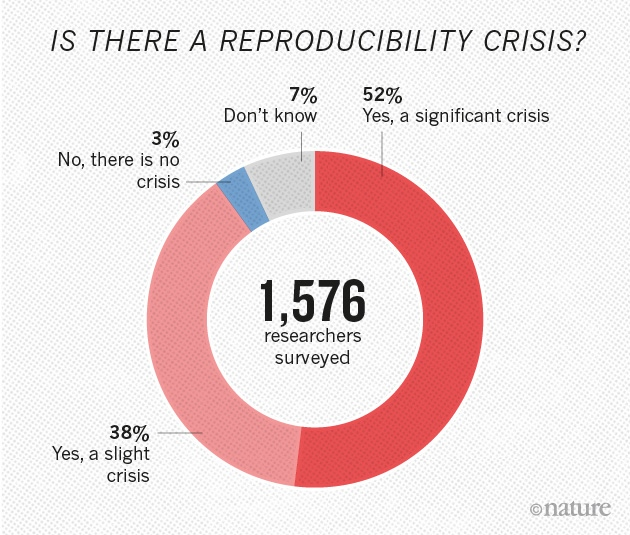
\includegraphics[height=.7\textheight]{figures/reproducibility-graphic-online1.jpeg}
        \caption{Is there a reproducibility crisis? \cite{Baker2016-cf}}
        \label{fig:Baker2016}
  \end{figure}
\end{frame}

\begin{frame}{Lost data}
 \begin{figure}[H]
    \centering
        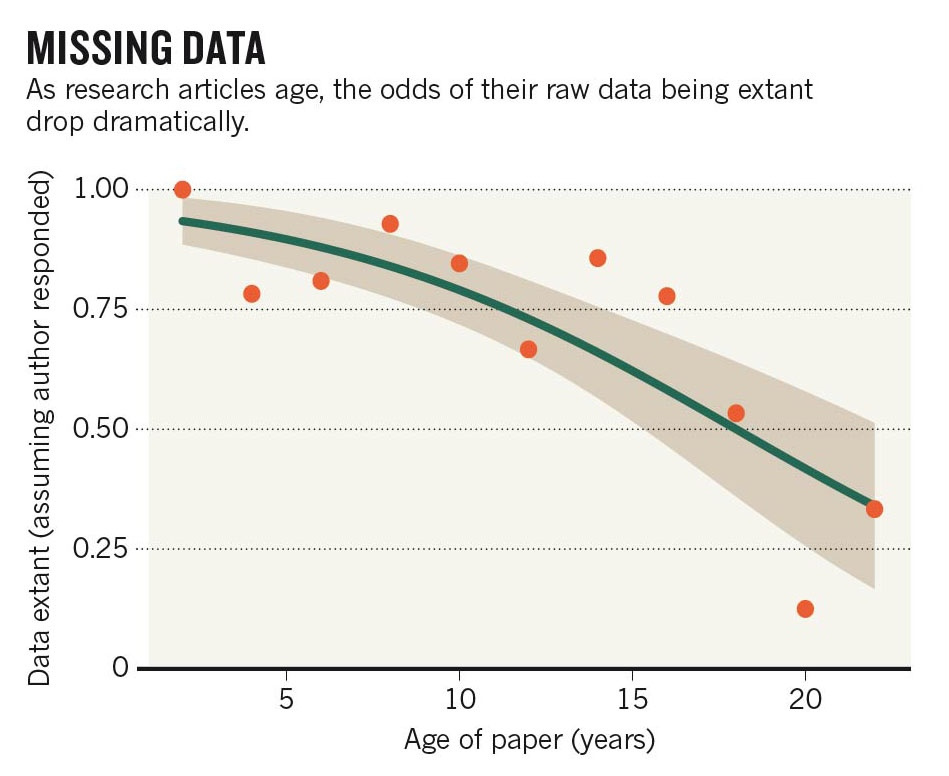
\includegraphics[height=.75\textheight]{figures/Missing-Data.png}
        \caption{\cite{Vines2014-zr}}
        \label{fig:vines2014}
 \end{figure}
\end{frame}

\begin{frame}{Calls for rigour and transparency}
  Manifestos, statements, and guidelines:
    \begin{itemize}[label=\textbullet]
        \item Early example: OECD Priniples and Guidelines for Access to Research Data \cite{Oecd2007-vi}.
        \item Findable, Accessible, Interoperable, and Reusable (FAIR) data \cite{Wilkinson2016-mr, Go-fair2017-vs}.
        \item Transparency and Openness Promotion (TOP) guidelines \cite{Nosek2015-wm, Cos2019-mr}.
        \item Data transparency toolkit \cite{Perkel2018-rw}.
    \end{itemize}
\end{frame}

\section{FAIR data mandates}

\begin{frame}{Journal transparency mandates}
  Mandates for transparency or reproducibility:
    \begin{itemize}[label=\textbullet]
        \item Nature: Transparency Upgrade \cite{Nature2017-lq}.
        \item Nature: FAIR data in Earth science \cite{Nature2019-ng}.
        \item Copernicus: FAIR data in atmospheric sciences \cite{Van_Edig2018-bu}.
        \item TOP Guidelines signatories include publishers representing 1000+ journals, as well as professional organisations and major private foundations  \cite{Cos2019-mr}.
    \end{itemize}
\end{frame}

% https://tex.stackexchange.com/a/2292/5483
% https://ctan.org/pkg/enumitem?lang=en

\begin{frame}{Level 2 TOP Guidelines for authors}
  
    \begin{enumerate}[label=\arabic*.]
        \setcounter{enumi}{1}
        % This increments the enumerate counter by 1.
        
        \item Authors using original data must:
        \begin{enumerate}[label=\alph*.]
            \item make the data available at a trusted digital repository [...]
            \item include all variables, treatment conditions, and observations described in the manuscript.
            \item provide a full account of the procedures used to collect, preprocess, clean, or generate the data.
            \item provide program code, scripts, codebooks, and other documentation sufficient to precisely reproduce all published results.
            \item provide research materials and description of procedures necessary to conduct an independent replication of the research.
        \end{enumerate}
    \end{enumerate}
    \cite{Osf2014-pf}
\end{frame}

\begin{frame}{TOP Guidelines: publisher adoption}
  \begin{figure}[H]
    \centering
        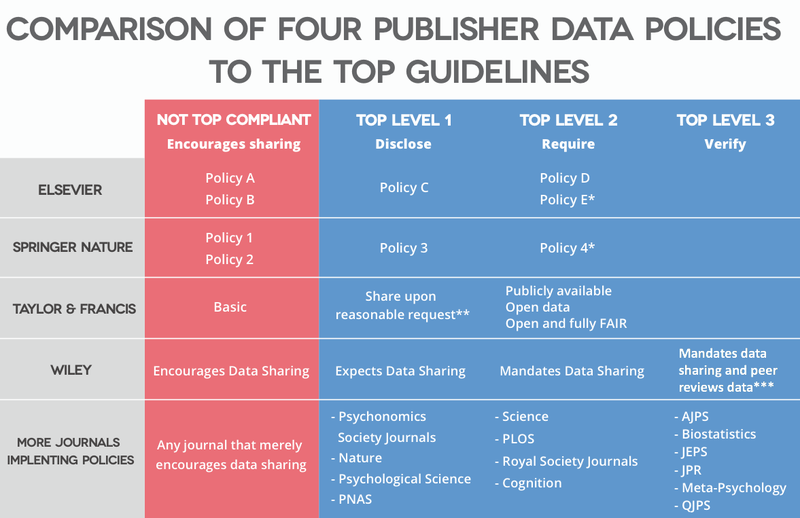
\includegraphics[height=.7\textheight]{figures/TOP-landscape.png}
        \caption{The Landscape of Open Data Policies \cite{Mellor2018-bf}}
        \label{fig:figure2}
  \end{figure}
\end{frame}

\begin{frame}{TOP Guidelines: funder endorsement}
  Private funders have endorsed via the Open Funders Research Group:
    \begin{itemize}[label=\textbullet]
        \item Alfred P. Sloan Foundation
        \item American Heart Association
        \item Bill and Melinda Gates Foundation
        \item Howard Hughes medical Institute
        \item John Templeton Foundation
        \item Laura and John Arnold Foundation
        \item Open Society Foundations
        \item Robert Wood Johnson Foundation
        \item Wellcome Trust
        \item and six more \cite{Ofrg2019-pq}
    \end{itemize}
\end{frame}

\begin{frame}{Other Funder data policies}
  \begin{figure}[H]
    \centering
        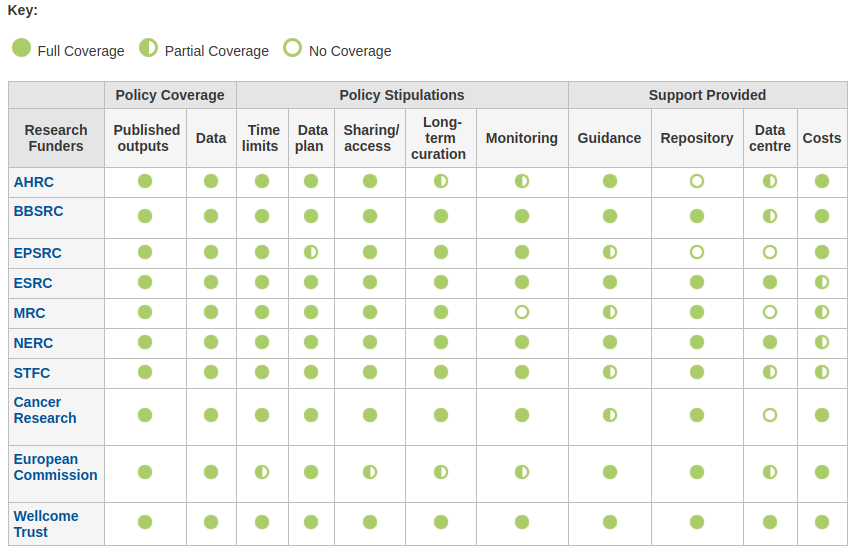
\includegraphics[height=.7\textheight]{figures/DCC-Funders.png}
        \caption{Overview of funders' data policies \cite{Dcc2019-jn}}
        \label{fig:Dcc2018}
  \end{figure}
\end{frame}

\begin{frame}{EU research governance policy}
  With the Horizon 2020 program \cite{European_Commission2019-an} Europe made `research data open by default':
    \begin{itemize}[label=\textbullet]
        \item `Participating projects will be required to develop a \textbf{Data Management Plan} (DMP), in which they will specify \textbf{what data will be open}: detailing \textbf{what data the project will generate}, whether and how it will be \textbf{exploited or made accessible for verification and re-use}, and how it will be \textbf{curated and preserved}.'
        \item Data should be `\textbf{as open as possible, as closed as necessary}'.
        \item Associated costs can be claimed in grant.
        \item Continuing investment, e.g., FAIRsFAIR project \cite{Knaw-dans2019-sv} to implement FAIR across repositories.
    \end{itemize}
\end{frame}

\begin{frame}{Not just the natural sciences}
  Changes are coming to HASS disciplines:
    \begin{itemize}[label=\textbullet]
        \item American Journal of Political Science requires (and tests) data and code \cite{Jacoby2017-lw, Ajps2015-ex}.
        \item Research Data Alliance (RDA) has an `Ambassador for the Humanities' and is examining how RDA standards and outputs can apply to humanities disciplines \cite{Rda2019-wc}.
        \item All European Academies (allea) E-Humanities working group \cite{Allea2019-wy} has issued an Open Consultation on `Sustainable and FAIR Data Sharing in the Humanities' \cite{Allea2019-aw}.
        \item Allea seeks to address the imperatives of the `Open Science agenda' across Humanities and Social Sciences, and `facilitate the adoption of Open Science across the Humanities'.
    \end{itemize}
\end{frame}

\begin{frame}{ALLEA report on FAIR Data in the Humanities }
  `Sustainable and FAIR Data Sharing in the Humanities' recommendations:
    \begin{itemize}[label=\textbullet]
        \item `Think of all your research assets as data...digitally document all your research and data collection work...use well-established tools...'
        \item `Devise a [Data Management Plan]...plan documentation of metadata...use standardised terminology...factor the cost of research data management'
        \item `Look for widely used formats possibly with documented standards....'
        \item `Use open standards...standardised technologies and procedures. prefer human and machine-readable systems...normalise as much as possible...'
        \item `Identify who owns the data...use free and standardised licences...make your licence machine-readable...'
        \item `Use disciplinary repositories where they exist...datasets should...include the richest metadata possible...'
        \item `Share online your data and all supporting materials...'
    \end{itemize}
\end{frame}

\begin{frame}{Challenges in HASS disciplines}
      \begin{itemize}[label=\textbullet]
        \item Copyright restrictions on texts, archival documents, films, audio recordings, secondary sources, etc.
        \item For evidence that is online, links and references possible (but access may have a cost, and links may die); if not online, the tyranny of distance re-asserts itself (if access is possible at all). 
        \item Socio-technical: training and expertise mismatch, \textbf{up-front time investment}, costs of suitable infrastructure and willingness to budget for them.
        \item Technical: `small data' problems, including diverse data; data and methods often emerge from research; just as hard as `big data', requires flexible and extensible infrastructure from a poorly coordinated and poorly funded domains \cite{Borgman2015-rh, Rda2019-wc}.
        \cite{Mons2020-tb}.
    \end{itemize}
\end{frame}

\section{Beyond compliance: improving research}

\begin{frame}{Avoiding `technical debt' and boring work}
    Too often in humanities research we settle for generic tools that are not a very good fit for what we actually need to do. 
        \begin{itemize}[label=\textbullet]
            \item Spreadsheets, though ubiquitous in research, are rarely a good idea
            \item Manual image management (renaming, etc.) takes a lot of time.
            \item Using several different tools, one each for structured data, images, geospatial data, etc., requires a lot of reconciliation time.
            \item The commonality is \textbf{technical debt}: trading quick setup for lengthy digitisation, cleaning, reconciliation, streamlining later.
            \item Let computers do the boring things that people are bad at, so that you can focus on the interesting parts of research.
    \end{itemize}
\end{frame}



\begin{frame}{Scaling your research}
    The same approaches that facilitate transparency and reproducibility support the kind of scalable and synthetic research that can address archaeological `grand challenges'. \cite{Kintigh2014-ub}
        \begin{itemize}[label=\textbullet]
            \item Paper data capture and manual digitisation and cleaning don't scale.
            \item Collaboration based on email and desktop software doesn't scale.
    \end{itemize}
\end{frame}

\begin{frame}{Scalable approaches to data and analysis}
  \begin{figure}[H]
    \centering
        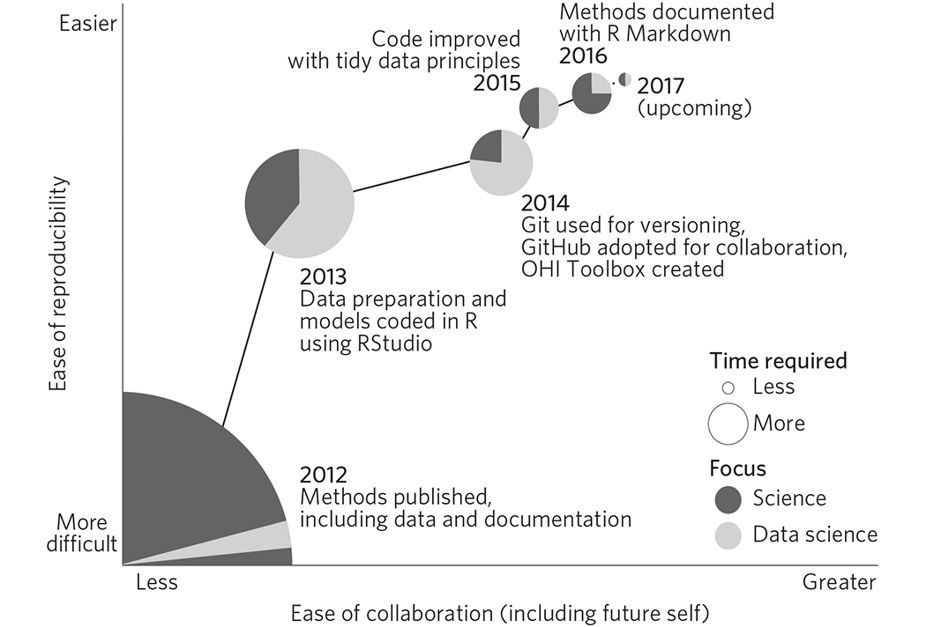
\includegraphics[height=.7\textheight]{figures/Ocean-Health-Index.jpg}
        \caption{Better science in less time, illustrated by the Ocean Health Index project. \cite{Stewart_Lowndes2017-lj}}
        \label{fig:stewart_lowndes}
  \end{figure}
\end{frame}

\begin{comment}

\section{From current practice to better practice}

\begin{frame}{What does this mean? Are we ready?}
  Emerging good practice - and publisher and funder policies - mean:
    \begin{itemize}[label=\textbullet]
        \item Comprehensive, FAIR datasets will be deposited in domain-specific repositories. Data, and especially metadata, quality will be higher.
        \item Data will be captured digitally as early in research as possible, and provenance / version history maintained.
        \item Research approach, processes, and procedures will be documented.
        \item Data processing and analysis will use code (not Excel!) 
        \item Code will be documented and published for reuse.
        \item Further steps taken for analytical reproducibility (use of OSS, version control, automation, containerisation, etc.). 
    \end{itemize}
\end{frame}

\begin{frame}{Challenges and paths forward}
  How do we get from where we are now to where we want to be?
      \begin{itemize}[label=\textbullet]
        \item Understand the evolving expectations of transparent research. 
        \item Pursue proper training
        \item Look past desktop software (Excel, ARCGIS, Filemaker, Access, etc.).
        \item Use emerging research- and domain-specific solutions (even if imperfect).
        \item Overcome `not invented here'; if a solution exists, use it.
        \item Budget for `ground-up' transparency (data and code). Up-front costs will be high but offer longer-term payoffs (in costs, time, and quality).
        \item Implement (and budget for) fundamental good practice in data and code management before other technologies.
        \item Improve research design (prioritise approach over methods) \cite{Muthukrishna2019-kt, Hole1973-cy}
    \end{itemize}
\end{frame}

\end{comment}

\section{`Small data' infrastructure across the data lifecycle}

\begin{frame}{`Small data' research}
 \begin{figure}[H]
    \centering
        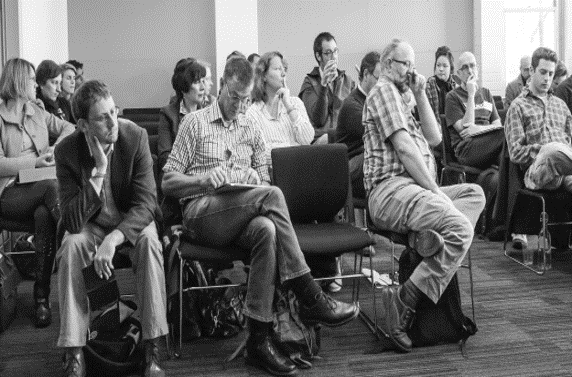
\includegraphics[height=.75\textheight]{figures/Archaeologists-standards.png}
        \caption{Archaeologists contemplate data standards (FAIMS Stocktaking, 2012)}
        \label{fig:figure7}
 \end{figure}
\end{frame}

\begin{frame}{Context: the challenge of `small data'}
    `Long tail' research: most field data is small data \cite{Borgman2015-rh}
    \begin{itemize}[label=\textbullet]
        \item Smaller scale; smaller communities; local control.
        \item Diverse questions, approaches, and methods.
        \item Heterogeneous data; variety of content, structure.
        \item Data and infrastructure emerge from fieldwork. 
        \item Relative lack of standards.
        \item Limited infrastructure and funding.
        \item Challenges associated with big(ger) data from photogrammetry, SfM, video, geophysics, etc., will exacerbate these problems.
    \end{itemize}
\end{frame}

\begin{frame}{The data lifecycle}
 \begin{figure}[H]
    \centering
        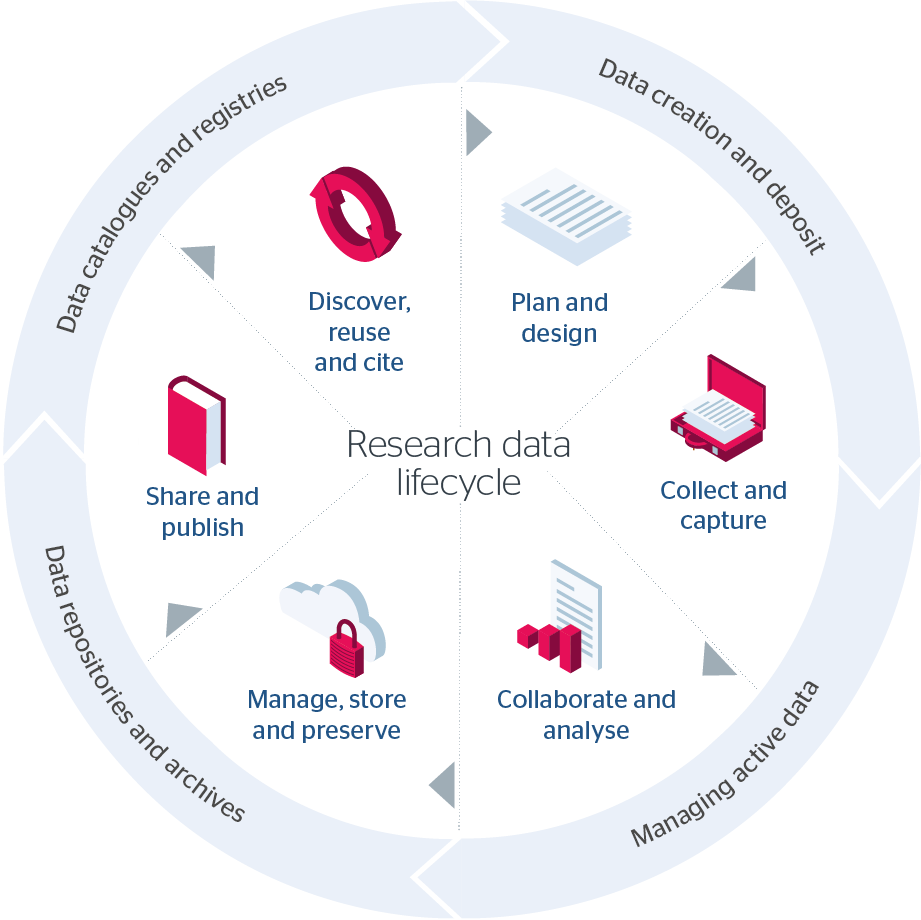
\includegraphics[height=.75\textheight]{figures/research-data-life-diagram.png}
        \caption{\cite{Jisc2018-gx} Image CC-BY-ND}
        \label{fig:figure9}
 \end{figure}
\end{frame}

\begin{frame}{Infrastructure across the data lifecycle}
    Consider the infrastructure needed to manage the three main phases of the data lifecycle
    \begin{itemize}[label=\textbullet]
        \item Publication (most mature): domain-specific repositories.
        \item Processing and analysis (less mature): project-level code \cite{Stewart_Lowndes2017-lj}, then Virtual Labs / Science Gateways, \cite{Alveo2019-tk}.
        \item Capture (least mature): most varied, needs to work offline under difficult conditions. Existing commercial solutions insufficient \cite{Bureau_of_Reclamation2017-xl}.
    \end{itemize}
\end{frame}

\section{The FAIMS approach}

\begin{frame}{Research Specific}
 \begin{figure}[H]
    \centering
        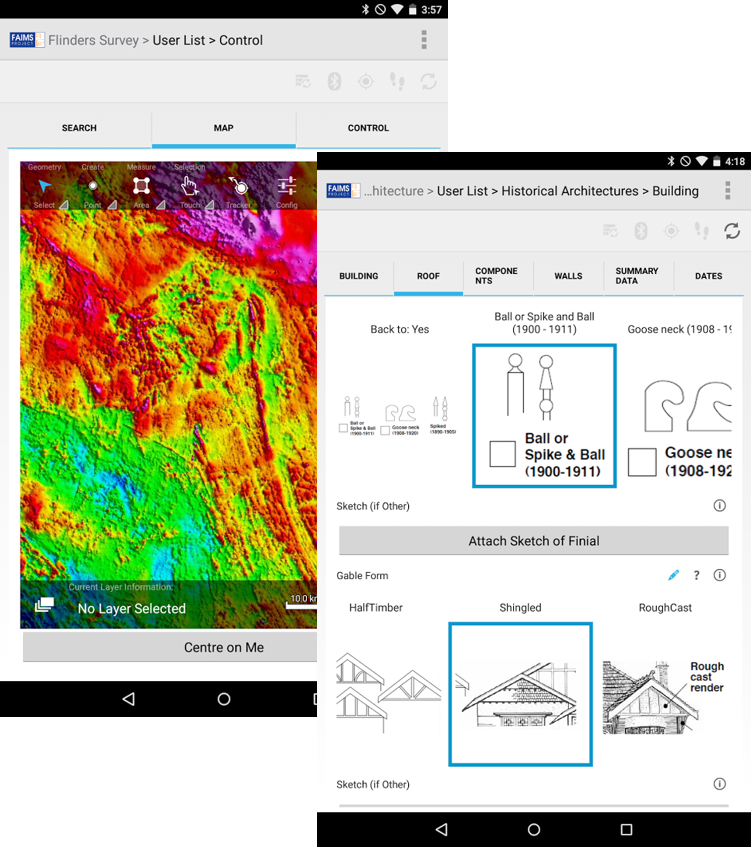
\includegraphics[height=.75\textheight]{figures/FAIMS-screenshots.png}
        \caption{FAIMS Mobile: GIS and `picture dictionaries'}
        \label{fig:FAIMS-mobile-screenshots}
 \end{figure}
\end{frame}

\begin{frame}{Key research-specific FAIMS Mobile features}
    \begin{itemize}[label=\textbullet]
        \item Fundamentally customisable (interpreter + definition files).
        \item Tightly binds structured, geospatial, multimedia, and free text data.
        \item Offline first, with automated bi-directional synchronisation.
        \item Record history: append-only datastore, versioning, rollback.
        \item Mobile GIS.
        \item Multimedia management (e.g., file renaming from record content).
        \item Connects to internal and external sensors, Bluetooth / USB devices.
        \item Multilingual.
        \item Granular help.
        \item Granular metadata.
        \item Generalised export.
        \item `Hooks’ for data interoperability, Open Linked Data approaches.
    \end{itemize}
\end{frame}

\begin{frame}{Generalised}
 \begin{figure}[H]
    \centering
        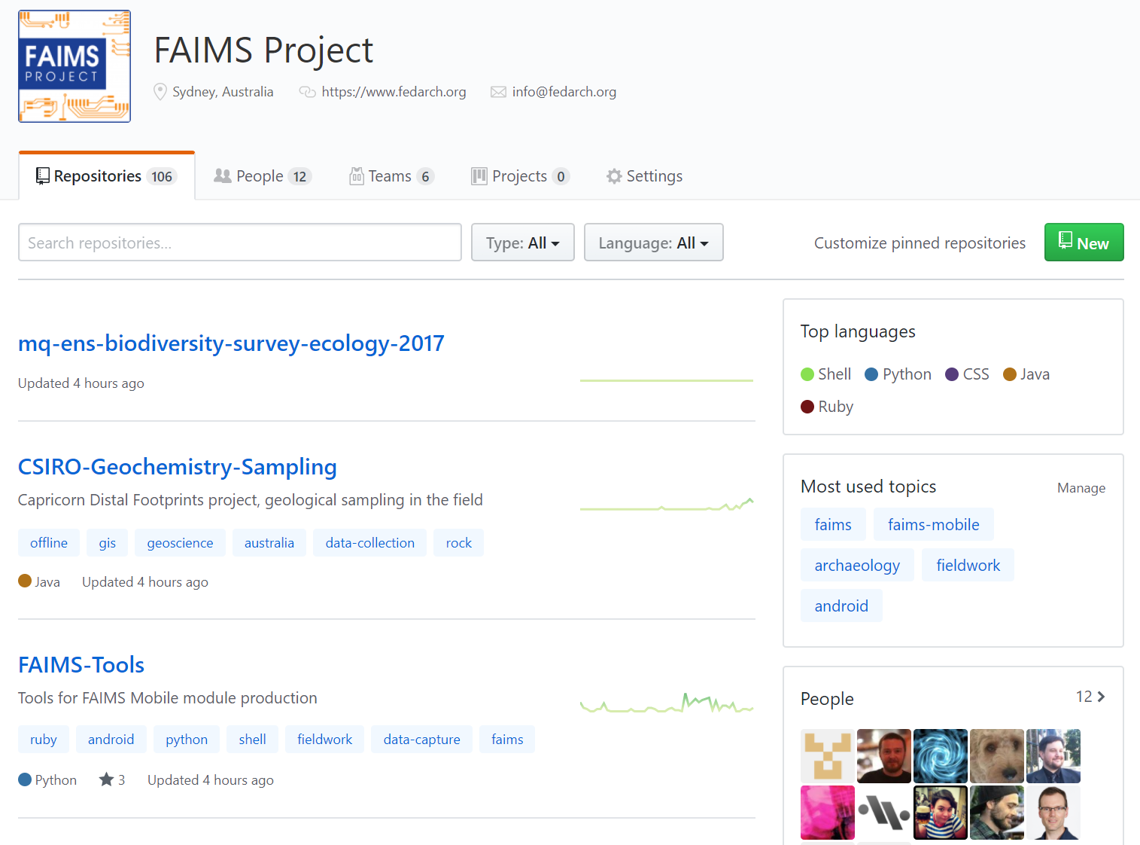
\includegraphics[height=.75\textheight]{figures/FAIMS-generalised.png}
        \caption{FAIMS Mobile customisations on GitHub}
        \label{fig:FAIMS-github}
 \end{figure}
\end{frame}

\begin{frame}{Modular and federated}
 \begin{figure}[H]
    \centering
        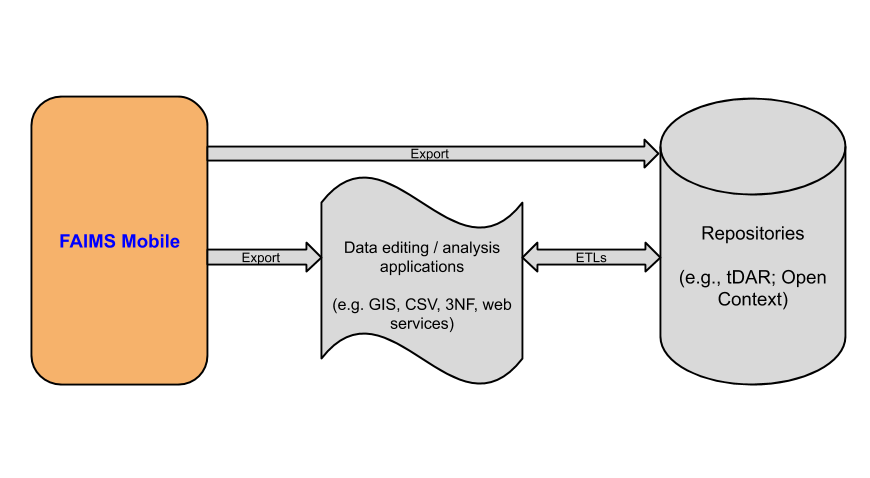
\includegraphics[height=.75\textheight]{figures/FAIMS-federation}
        \caption{FAIMS Mobile federation}
        \label{fig:FAIMS-federation}
 \end{figure}
\end{frame}

\begin{frame}{Open Source}
 \begin{figure}[H]
    \centering
        
\includegraphics[width=.75\textwidth]{figures/GPLv3_Logo.eps}
        \caption{FAIMS Mobile `core' code is GPLv3; `module' (customisation) code is also open; everything is on GitHub}
        \label{fig:FAIMS-github-OSS}
 \end{figure}
\end{frame}

\begin{frame}{Status and plans for the future}
    \begin{itemize}[label=\textbullet]
        \item FAIMS v2.6 is nearing end of its useful life.
        \item A high-level technical plan for FAIMS v3.0 won a US design prize in 2017 \cite{Bureau_of_Reclamation2017-xl}.
        \item Any future iteration of FAIMS must be sustainable via commercialisation as a (primarily) self-service platform.
        \item The FAIMS team did CSIRO ON Prime in 2016, completing 70+ interviews with clients / potential clients.
        \item \textbf{We have won a \$600k ARDC Platforms grant to rebuild FAIMS.}
        \item Challenges: sustainability, uptake (overcoming resistance initial setup investment; overcoming resistance to cost), balancing open research requirements against commercialisation demands.
    \end{itemize}
\end{frame}

\begin{frame}{Planned technical improvements}
User / potential user interviews drive technical improvements, which aim to make deployment and use easier, increasing update.
    \begin{itemize}[label=\textbullet]
        \item Cross-platform support (Android; iOS; desktop)
        \item Self-customisation by the user via a GUI-based web application.
        \item Orchestrated deployment of infrastructure to (e.g.) Amazon Web Services.
        \item Data `round-trip' to desktop or online software.
        \item Exposure of data via an API
        \item Improved scalability (application performance; synchronisation performance; server-to-server synchronisation)
        \item Improved user management and security
    \end{itemize}
\end{frame}

\begin{comment}

\begin{frame}{Selected FAIMS Testimonials}
    \begin{itemize}[label=\textbullet]
    \item ``The tablet app worked very well in the field and I would be keen to continue using it for subsequent sampling'' -- New Zealand Soil Geochemistry
    \item ``Being able to check in on everyone's work from my computer so easily is... revolutionary. Thank you for building such an amazing tool! …  I look forward to providing more details, but I already feel like I have 100\%{} better control over data quality, even compared to last year'' -- Proyecto Arquelogico de Zana Colonial
    \end{itemize}
\end{frame}

\begin{frame}{Selected FAIMS Testimonials 2}
    \begin{itemize}[label=\textbullet]
    \item ``The app has been such an incredible advantage in terms of workload, data quality, and a number of other data management issues with which archaeologists regularly have to deal. It readily links disparate data types that are otherwise stored separately – such as photographs, tabular logs, and context relationships.'' -- Malawi Early-Middle Stone Age Project
    \item ``I was really impressed with the approach FAIMS project has taken to the challenge of creating field data apps which can be very expensive. Our module was ready for testing after just one briefing.'' -- Streamwatch
    \end{itemize}
\end{frame}

\begin{frame}{Selected FAIMS Testimonials 3}
    \begin{itemize}[label=\textbullet]
\item 
``We’re back from the field and I cannot believe how well everything went. ... [T]he combination of the mobile lab, the sample ID/tracking and FAIMS application enabled us to average 5-6 minutes per sample site (crust, soil, rock and two plants)  in the field and about half that in the lab... Using the old school notepad and GPS approach this would have been 15 mins at best and a whole lot of misplaced photos and details, not to mention the additional hours entering the data in at night. We were able to identify missed sites as we went and completed the soils map (280 sites) and infill (36 sites) and analysis all in the 7 days. '' -- CSIRO Mineral Resources
\end{itemize}
\end{frame}

\begin{frame}{Status and plans for the future}
    \begin{itemize}[label=\textbullet]
        \item FAIMS v2.6 is nearing end of its useful life.
        \item A high-level technical plan for FAIMS v3.0 won a US design prize in 2017 \cite{Bureau_of_Reclamation2017-xl}.
        \item Any future iteration of FAIMS must be sustainable via commercialisation as a (primarily) self-service platform.
        \item The FAIMS team did CSIRO ON Prime in 2016, completing 70+ interviews with clients / potential clients.
        \item We are considering applying for an ARDC Platforms and Services grant, if we can reconcile that with commercialisation.
        \item Challenge: balancing open research / OSS with commercialisation.
    \end{itemize}
\end{frame}

\begin{frame}{Technical improvements}
    \begin{itemize}[label=\textbullet]
        \item Cross-platform support (Android; iOS; desktop)
        \item Self-customisation by the user via a GUI-based web application.
        \item Orchestrated deployment of infrastructure to (e.g.) Amazon Web Services.
        \item Data `round-trip' to external desktop or online software.
        \item Exposure of data via an API
        \item Improved scalability (application performance; synchronisation performance; server-to-server synchronisation)
        \item Improved user management and security
    \end{itemize}
\end{frame}

\end{comment}

\begin{frame}{FAIMS publications}
Available at: \url{https://paperpile.com/shared/yk95gS}

      \begin{itemize}[label=\textbullet]
      
      
      {\small
      \nocite{Sobotkova2015-lq,Sobotkova2018-al,VanValkenburgh2018-hv,Ballsun-Stanton2018-zd,Sobotkova2016-mx,Ross2015-ph,Ross2013-hi}
        % \item \nocite{Sobotkova2018-al}
        % \item \nocite{Ballsun-Stanton2018-zd}
        % \item \nocite{VanValkenburgh2018-hv}
        % \item \nocite{sobotkova2016-mx}
        % \item \nocite{Ross2015-ph} 
        % \item \nocite{Sobotkova2015-lq}
        % \item \nocite{Ross2013-hi}
\item Ballsun-Stanton, Brian, Shawn A. Ross, Adela Sobotkova, and Penny Crook. 2018. ``FAIMS Mobile: Flexible, Open-Source Software for Field Research.''
\item Ross, Shawn Adrian, Brian Ballsun-Stanton, Adela Sobotkova, and Penny Crook. 2015. ``Building the Bazaar: Enhancing Archaeological Field Recording Through an Open Source Approach.''
\item Ross, Shawn Adrian, Adela Sobotkova, Brian Ballsun-Stanton, and Penny Crook. 2013. ``Creating Eresearch Tools For Archaeologists: The Federated Archaeological Information Management Systems Project.''
\item Sobotkova, Adela. 2018. ``Sociotechnical Obstacles to Archaeological Data Reuse.'' 

}
    \end{itemize}
\end{frame}

\begin{frame}{FAIMS Publications 2}
\begin{itemize}[label=\textbullet]
{\small
    \item Sobotkova, Adela, Brian Ballsun-Stanton, Shawn Ross, and Penny Crook. 2015. ``Arbitrary Offline Data Capture on All of Your Androids: The FAIMS Mobile Platform.''
\item Sobotkova, Adela, Shawn A. Ross, Brian Ballsun-Stanton, Andrew Fairbairn, Jessica Thompson, and Parker VanValkenburgh. 2016. ``Measure Twice, Cut Once: Cooperative Deployment of a Generalized, Archaeology-Specific Field Data Collection System.'' 
\item VanValkenburgh, Parker, Luiza O. G. Silva, Chiara Repetti-Ludlow, Jake Gardner, Jackson Crook, and Brian Ballsun-Stanton. 2018. ``Mobilization as Mediation: Implementing a Tablet-Based Recording System for Ceramic Classification.''} 
\end{itemize}
    
\end{frame}
\begin{frame}{Thank you!}

%This presentation is available at:
%\texttt{https://osf.io/v5jp7/}

PDF and source code for this presentation is available at: 
\texttt{https://github.com/saross/FAIMS-for-HASS/releases/tag/v1.0}

FAIMS Project software and documentation can be found at:
\texttt{https://github.com/faims}.

This work is licensed under a Creative Commons Attribution 4.0 International License.

\end{frame}

% \bibliographystyle{apalike}

% Adding the option 'allowframebreaks' allows the contents of the slide to be expanded in more than one slide.
% The "1" comes from the outer theme"

\section{References}

\begin{multicols}{2}[]
\bibliography{references}
\bibliographystyle{apalike}
\end{multicols}


% \begin{frame}[allowframebreaks]{References}
  
%   \bibliography{references}
%   \bibliographystyle{apalike}
% \end{frame}

\end{document}